\section{Introduction}
\label{sec:introduction_chip}

The cost of \gls{SNP} arrays have declined over the years. This has made it possible to increase study sizes at a fixed budget. However, most current \gls{SNP} arrays do not capture variation in African populations well. As shown in table \ref{tab:chip_SNPs} on page \pageref{tab:chip_SNPs}, figure \ref{fig:SN02f2} and elsewhere\cite{Gurdasani2015} approximately 20\% of the autosomal SNPs on the Illumina HumanOmni2.5 SNP array are monomorphic in African populations. And as shown in figure \ref{fig:SN10f2} on page \pageref{fig:SN10f2} \gls{SNP} density also alters imputation accuracy quite significantly. And SN2 figure 2 on page 58 of the supplementary material to the AGV project publication\cite{Gurdasani2015} shows that the site frequency spectrum on the Omni2.5 array in 3 African populations has ascertainment bias by being skewed towards common variants. Therefore it is desirable to explore whether a continent specific \gls{SNP} array can capture variation in African populations better. I do so here. This work should be seen in relation to the results on page \pageref{sec:rp_results} showing that common variation is captured well relative to low coverage sequencing, when continent specific reference panels are used. The development of continent specific reference panels and \gls{SNP} arrays could possibly be a great combination that could compete with study designs involving sequencing. I refer to the \gls{SNP} array as hypothetical here, because no manufacturer has confirmed, that the selected tag \glspl{SNP} are viable to go on a \gls{SNP} array. But by using nearby \glspl{SNP} that can be assayed it should be possible to achieve results very comparable to those presented here.

\begin{figure}
\centering
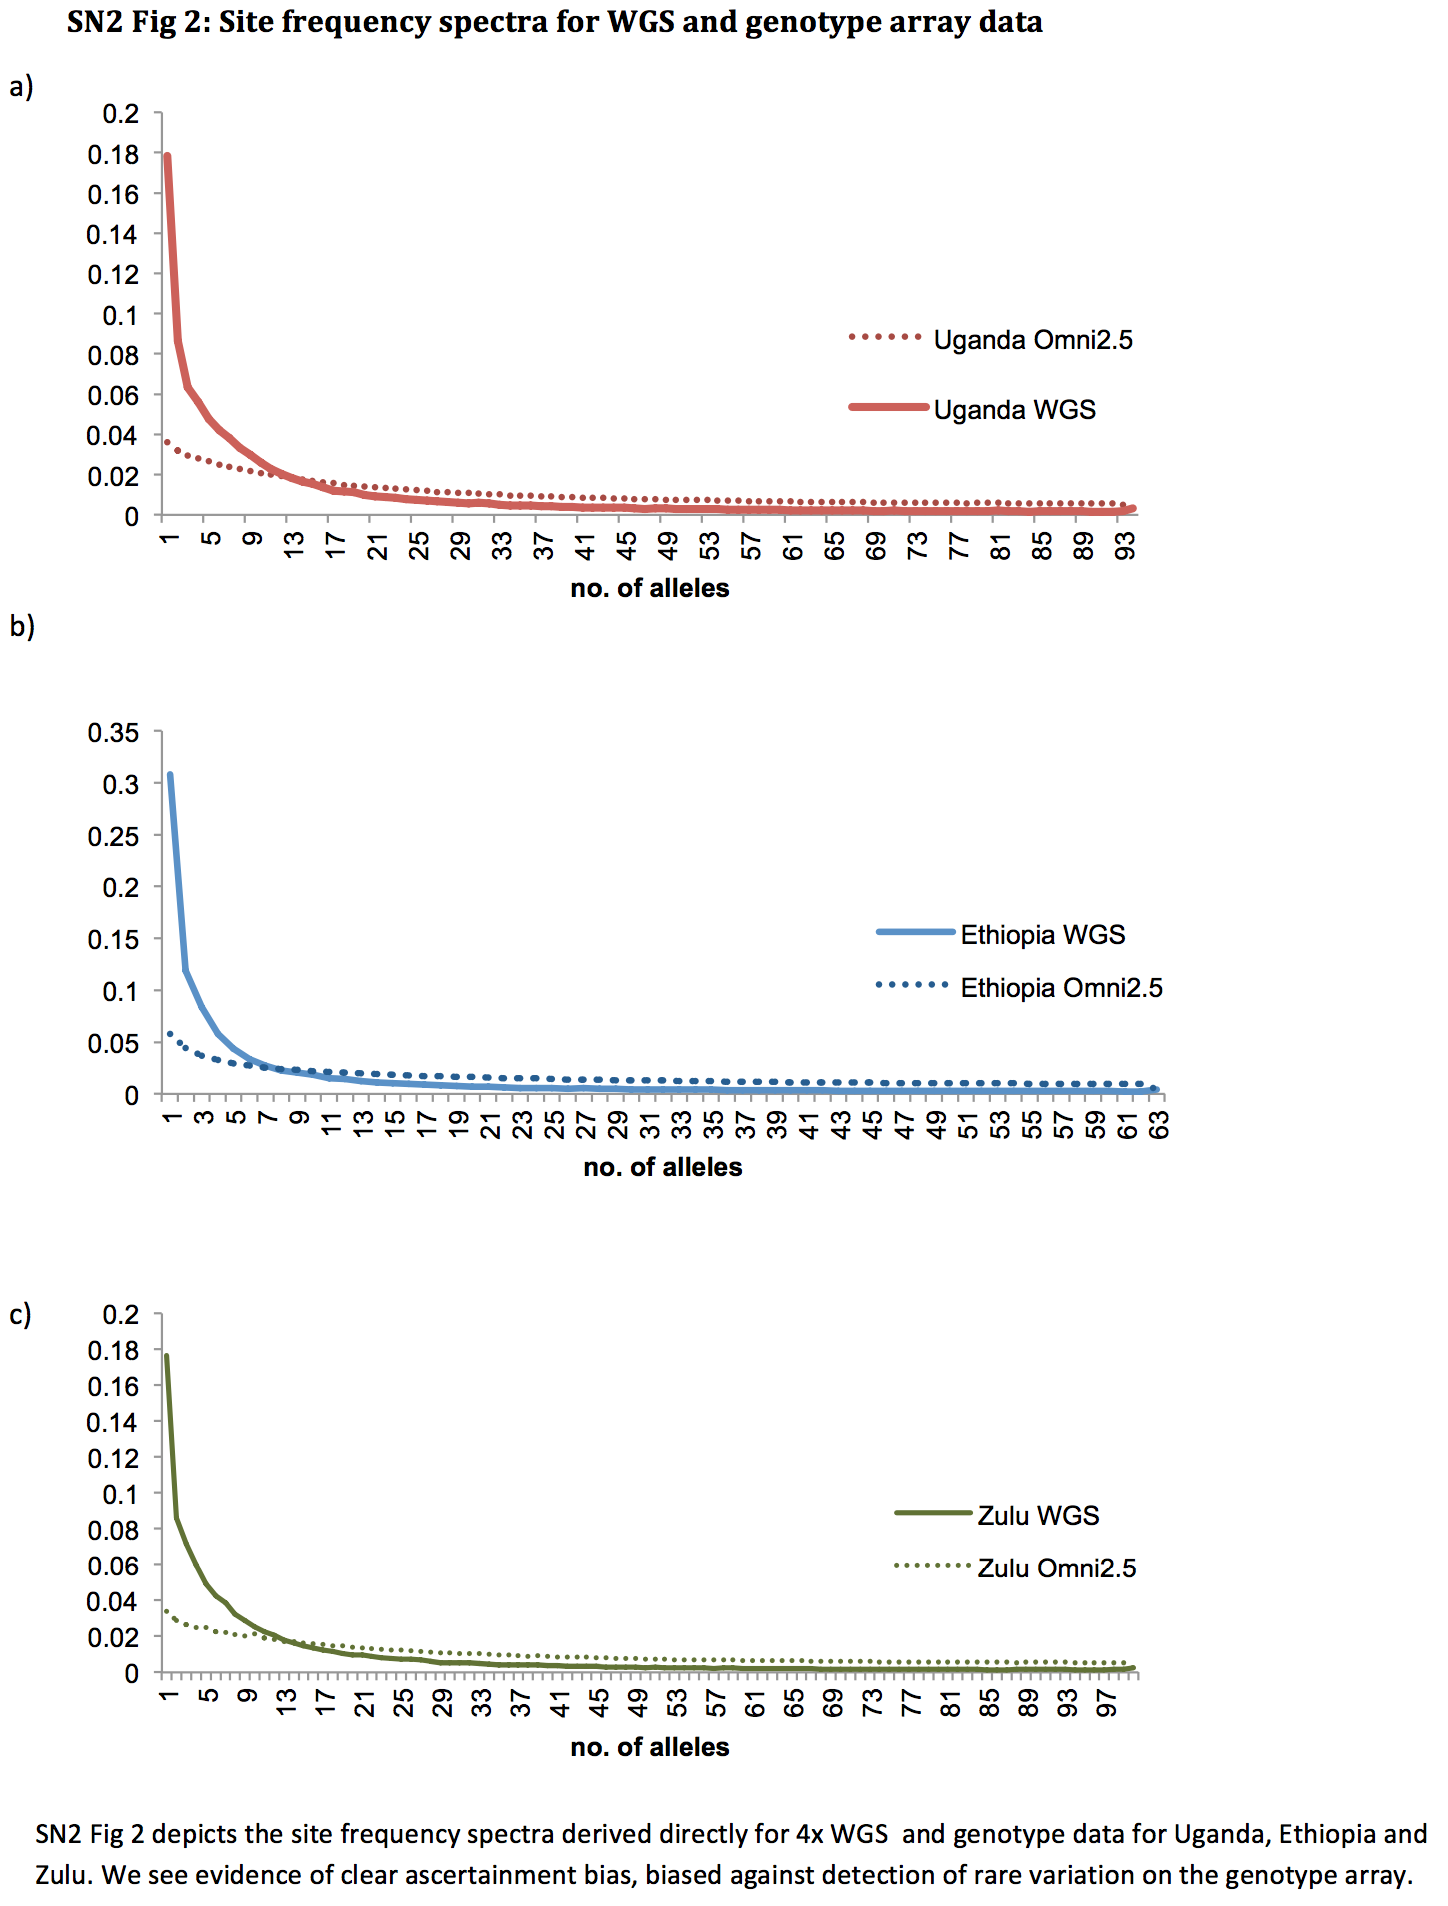
\includegraphics[trim={0 2cm 4cm 1cm},clip,width=0.8\textwidth]{fig/SN02f2}
\caption[Site frequency spectrum of sequence and SNP array data]{Site frequency spectrum derived directly from 4x \gls{WGS} data and SNP array data for the populations Uganda, Zulu and Ethiopia. Ascertainment bias against detection of rare variation on the SNP array is seen. On the x-axis is the number of alleles. On the y-axis is the relative frequency for each allele count.}
\label{fig:SN02f2}
\end{figure}
